% \documentclass{article}
\documentclass{mycv}

\usepackage[margin=2.0cm,right=3cm]{geometry}
\usepackage{paracol,xcolor,lipsum}
\usepackage{graphicx}
\usepackage{fontawesome}
\usepackage[english]{babel}
\usepackage[T1]{fontenc}
%\usepackage{tgheros} % or helvet
% \usepackage[scale=.9]{tgheros} % or helvet

\usepackage[scaled]{helvet}
\renewcommand\familydefault{\sfdefault}
%\usepackage[T1]{fontenc}

\usepackage{multirow}
\usepackage{hyperref}

\hypersetup{hidelinks=true}

\begin{document}
\pagenumbering{gobble}
\urlstyle{sf}
\columnratio{0.3,0.03}
\begin{paracol}{3}

  %% \backgroundcolor{c[2]}[rgb]{0.0,0,0}

  \begin{figure}[h!]
    \centering
    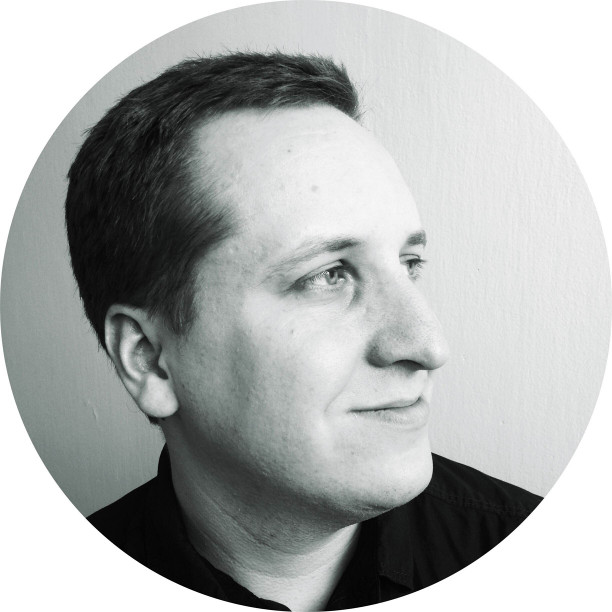
\includegraphics[width=0.8\linewidth]{img/prof3_lq.jpg}
    %% \includegraphics[width=0.5\linewidth]{img/prof1.jpg}
    %%    \includegraphics[width=2cm]{img/avatar.png}
  \end{figure}

  \vspace{1cm}
  %% \topic{Info}{\faInfo}
  %% \vspace{2mm}

  \leftline{
    \begin{tabular}{cl}
      \multirow{2}{*}{\large{\faMale}} & \textsc{\large{Name}} \\
      &  Pavel Reichl \\
      \multirow{0}{*}{} & \\
      \multirow{3}{*}{\large{\faMapMarker}} & \textsc{\large{Address}} \\
      &  Brno \\
      &  Czech Republic \\
      \multirow{0}{*}{} & \\
      \multirow{1}{*}{\large{\faEnvelopeO}} & \textsc{\large{Email}} \\
      & \small{\url{reichl.pavel@gmail.com}} \\
      \multirow{0}{*}{} & \\
      \multirow{1}{*}{\large{\faMobile}} & \textsc{\large{Phone}} \\
      & +420 777 983 828 \\
      \multirow{0}{*}{} & \\
      \large{\faLinkedin} & \textsc{\large{Linkedin}} \\
      \multicolumn{2}{l}{\small{\url{cz.linkedin.com/in/pavelreichl}}} \\
    \end{tabular}
  }

\vspace{10mm}

\topic{Profile}{\faFileO}

{\small{
    I am a software engineer interested in system and security software and also generally in Linux programming, and open source. I have a background of a game developer which gave me experience with optimization and computer graphics. I am looking for new challenges.
  }
}

\vspace{10mm}

\topic{Languages}{\faFlagO}
\vspace{2mm}
\leftline{
  \begin{tabular}{rc}
    \textsc{\large{Czech}} & \multirow{2}{*}{\large{\faStar \faStar \faStar}} \\ Native \\
    \multirow{0}{*}{} & \\
    \textsc{\large{English}} & \multirow{2}{*}{\large{\faStar \faStar \faStarHalfO}} \\ Working Proficiency \\
    \multirow{0}{*}{} & \\
    \textsc{\large{German}} & \multirow{2}{*}{\large{\faStarHalfO \faStarO \faStarO}} \\ Elementary Proficiency
  \end{tabular}
}


\switchcolumn
\switchcolumn

%%%%%%%%%%%%%%%%%%%%%%%%%%%%%%%%%%%%%%%%%%%%%%%%%%%%%%%%%%%%%%%%%%%%%%%%%%%%%%%%
%% Right Page
%%%%%%%%%%%%%%%%%%%%%%%%%%%%%%%%%%%%%%%%%%%%%%%%%%%%%%%%%%%%%%%%%%%%%%%%%%%%%%%%

\leftline{
  \resizebox{0.8\linewidth}{!}{\textbf{Pavel Reichl}}
}

\vspace{4mm}

\leftline{
  \resizebox{0.55\linewidth}{!}{\textsc{Software engineer}}
}

\vspace{9mm}

%% Work experience  %%%%%%%%%%%%%%%%%%%%%%%%%%%%%%%%%%%%%%%%%%%%%%%%%%%%%%%%%%%%

\topic{Work Experience}{\faCogs}

\jobls{Oct 2013-–May 2016}{\redhat}{Brno}{Software engineer}{
Designing and developing new features with emphesis on product security and efficiency, code reviewing, bug fixing, testing, helping users and support engineers with troubleshooting, participating in planning and documentation processes.
}{
  C|Git|Fedora|LDAP|Kerberos|PAM|Autotools}

\mjobls{Sep 2011-–Jan 2013}{Seznam.cz}{Brno}{Tech team programmer}{
    Member of a tech team responsible for maintenance of corporate technology and development of new tools.
}{
  C++|Python|Git}{
  Programmer}{
  Maintenance of high-traffic web applications. (novinky.cz, sport.cz, super.cz)}{
  Python|SVN|Debian}

\jobls{Jun 2008-–Nov 2010}{\hammerware}{Brno}{Game Developer}{
    Development of cross-platform games -- programming, debugging, optimization and testing.
}{C++|SVN|Ogre}

\jobls{Jun 2007--Oct 2010}{Handjoy}{Brno}{Game Developer}{
    One time contract on a single project.
}{C++|OpenGL|SDL}

\topicend

%% Education %%%%%%%%%%%%%%%%%%%%%%%%%%%%%%%%%%%%%%%%%%%%%%%%%%%%%%%%%%%%%%%%%%%

\topic{Education}{\faMortarBoard}

\uni{2010--2013}{Masaryk University}{Brno}{Master's degree of Applied Informatics}{Procedural modelling of buildings}

\uni{2005--2008}{Masaryk University}{Brno}{Bachelor's degree of Applied Informatics}{Octree-based Ray Tracer}

\topicend

\topic{Projects}{\faFolderO}
\project{SSSD}{\redhat}{
  SSSD is a system daemon. Its primary function is to provide access to identity and authentication of remote resources.}{\faLinux\ \faLock}
\project{pam\_hbac}{\redhat}{
  A PAM account module that evaluates HBAC rules stored on an IPA server.}{\faLinux\ \faLock}
\project{Family Farm}{\hammerware}{
  Innovative sim/tycoon game in the setting of 19th century farmstead for PC, Mac and
  Linux.}{\faWindows\ \faGamepad}

\end{paracol}

\end{document}
